\section{4-bit Carry Look-ahead Adder(CLA) (augmented)}
Instead of creating the $c out$ in the 4-bit Carry Look-ahead Adder(CLA)  (augmented), we supply the block propagate(P) and generate(G) as signals, which are subsequently used by the look carry ahead unit. By utilising the block propagate(P) and generate(G) signals, we may create 16-bit, 32-bit, and 64-bit CLA  Augmented Adders using this modular logic design.
\subsection{Circuit Diagram}
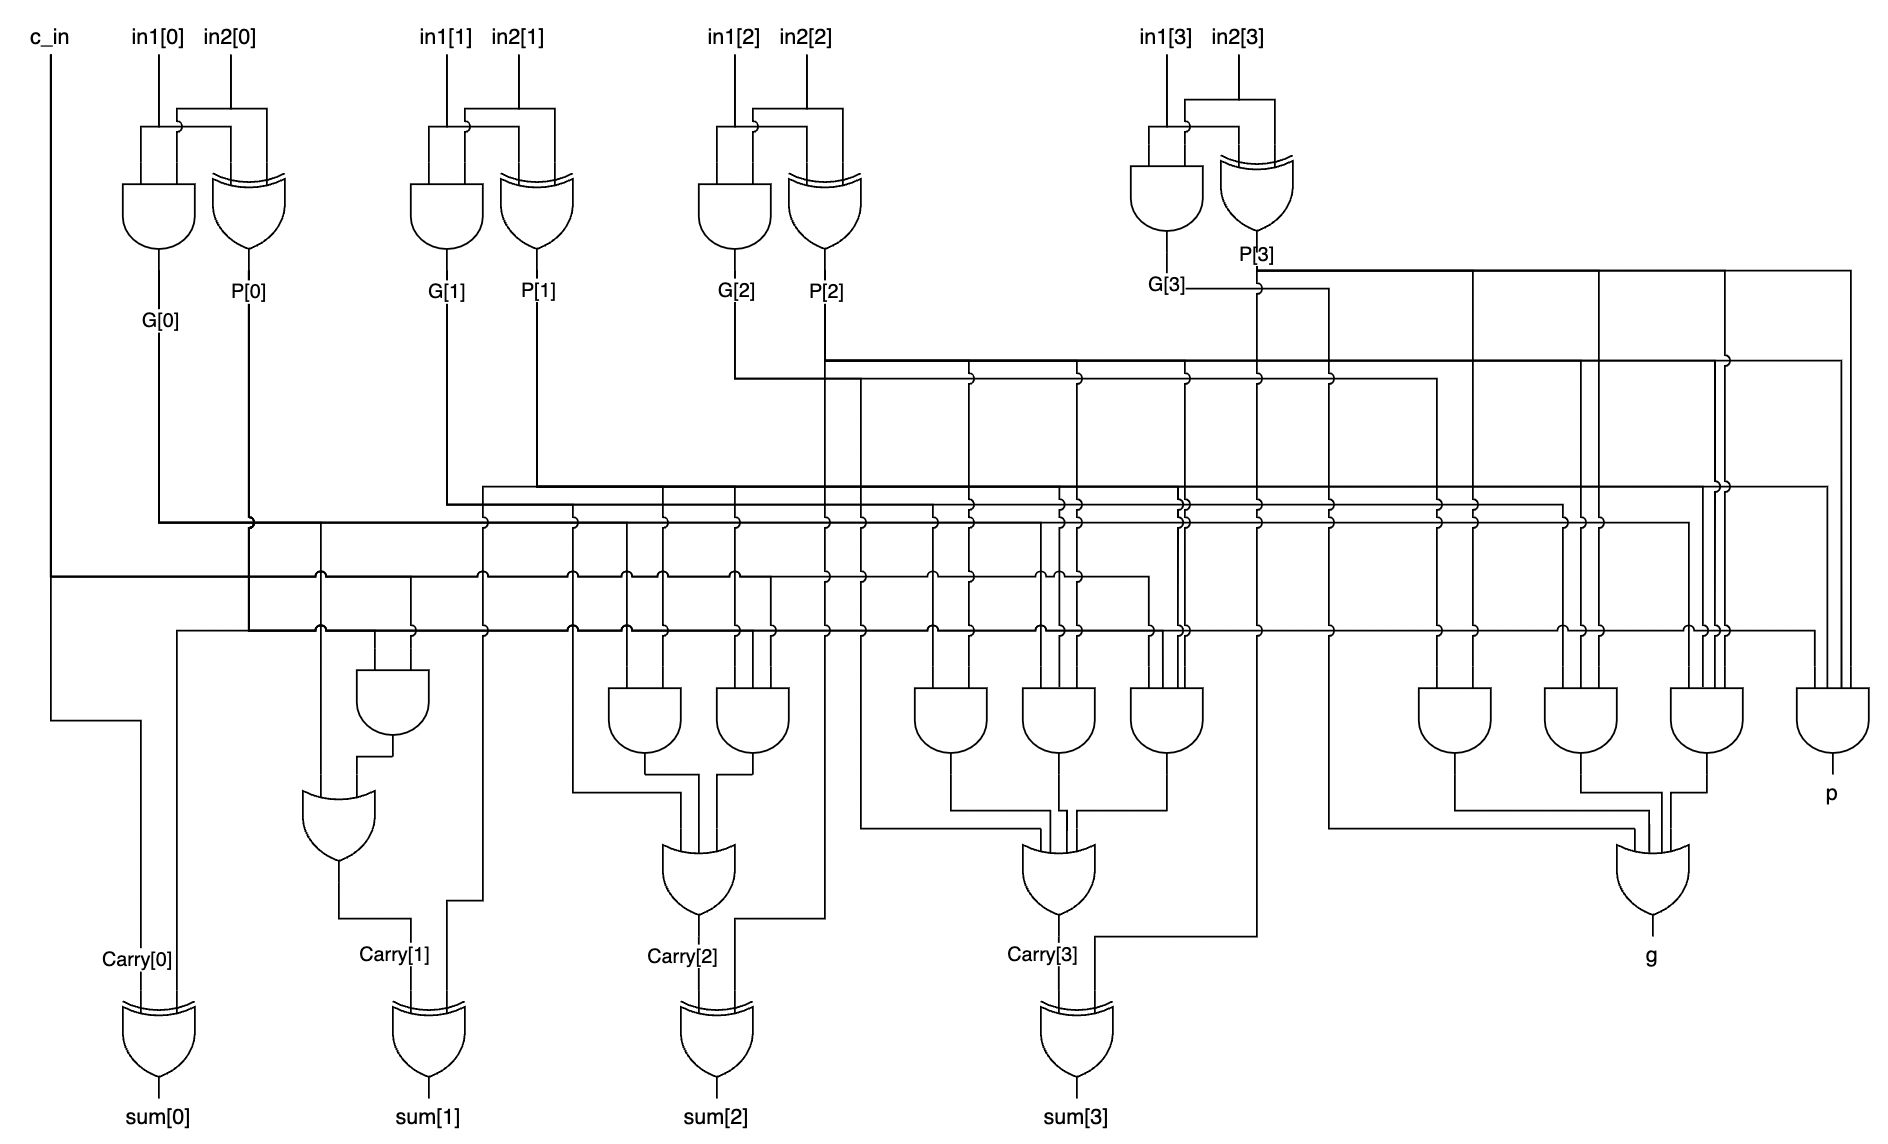
\includegraphics[width = 18cm]{images/cla_4_bit_aug.png}
\subsection{Logic Expression}
The Block Propagate and the Generate Signals are calculated as follows:-
\begin{equation} p = P[3] \And P[2] \And P[1] \And P[0]\end{equation}
\begin{equation} g = G[3] | (P[3] \And G[2]) | (P[3] \And P[2] \And G[1]) | (P[3] \And P[2] \And P[1] \And G[0]) )\end{equation}
